\documentclass[10pt, compress, xcolor={table,xcdraw}, aspectratio=169]{beamer}

\usetheme[numbering=fraction, progressbar=none, titleformat=smallcaps, sectionpage=none]{metropolis}

\usepackage{sourcecodepro}
\usepackage{booktabs}
\usepackage{array}
\usepackage{listings}
\usepackage{graphicx}
\usepackage[english]{babel}
\usepackage[scale=2]{ccicons}
\usepackage{url}
\usepackage{relsize}
\usepackage{wasysym}

\usepackage{pgfplots}
\usepgfplotslibrary{dateplot}

\definecolor{Base}{HTML}{191F26}
\definecolor{Accent}{HTML}{157FFF}

\setbeamercolor{alerted text}{fg=Accent}
\setbeamercolor{frametitle}{bg=Base}

\setsansfont[BoldFont={Source Sans Pro Semibold},
              Numbers={OldStyle}]{Source Sans Pro}

\lstset{ %
  backgroundcolor={},
  basicstyle=\ttfamily\footnotesize,
  breakatwhitespace=true,
  breaklines=true,
  captionpos=n,
  commentstyle=\color{Accent},
  escapeinside={\%*}{*)},
  extendedchars=true,
  frame=n,
  keywordstyle=\color{Accent},
  language=C++,
  rulecolor=\color{black},
  showspaces=false,
  showstringspaces=false,
  showtabs=false,
  stepnumber=2,
  stringstyle=\color{gray},
  tabsize=2,
  keywords={thrust,plus,device_vector, copy,transform,begin,end, copyin,
  copyout, acc, \_\_global\_\_, void, int, float, main, threadIdx, blockIdx,
  blockDim, if, else, malloc, NULL, cudaMalloc, cudaMemcpy, cudaSuccess,
  cudaGetLastError, cudaDeviceSynchronize, cudaFree, cudaMemcpyDeviceToHost,
  cudaMemcpyHostToDevice, const, data, independent, kernels, loop,
  fprintf, stderr, cudaGetErrorString, EXIT_FAILURE, for, dim3},
  otherkeywords={::, \#pragma, \#include, <<<,>>>, \&, \*, +, -, /, [, ], >, <}
}

\renewcommand*{\UrlFont}{\ttfamily\smaller\relax}

\graphicspath{{../img/}}

\title{Autotuning HLS for FPGAs using OpenTuner and LegUp}
\author{\footnotesize Pedro Bruel {\scriptsize (\emph{phrb@ime.usp.br})} \\
\footnotesize \textbf{Alfredo Goldman} {\scriptsize (\textbf{\emph{gold@ime.usp.br}})} \\
\footnotesize Sai Rahul Chalamalasetti {\scriptsize (\emph{gold@ime.usp.br})} \\
\footnotesize Dejan Milojicic {\scriptsize (\emph{gold@ime.usp.br})}}
\institute{
\includegraphics[height=1.8cm]{imelogo}\\[0.2cm] \emph{Institute of Mathematics and Statistics \\ University of São Paulo} \\[.2cm]  \hspace{.5cm} 
\includegraphics[height=.5cm]{cnpqlogo} \hspace{.5cm} 
\includegraphics[height=.75cm]{capeslogo_} \hspace{.5cm} 
\includegraphics[height=.58cm]{hpelogo}}
\date{\scriptsize ReConFig, December 5, 2017}

\begin{document}

\maketitle

\section*{Introduction}

\subsection*{About}

%\begin{frame}
%    \frametitle{About}
%    \begin{columns}[T,onlytextwidth]
%        \column{0.5\textwidth}
%        \begin{center}
%            
\includegraphics[width=.45\textwidth]{pedro}
%
%            Pedro Bruel \\
%            \emph{\alert{phrb}@ime.usp.br} \\[.3cm]
%            \url{www.ime.usp.br/~phrb} \\
%            \url{github.com/phrb} \\
%        \end{center}
%
%        \column{0.5\textwidth}
%        \begin{center}
%            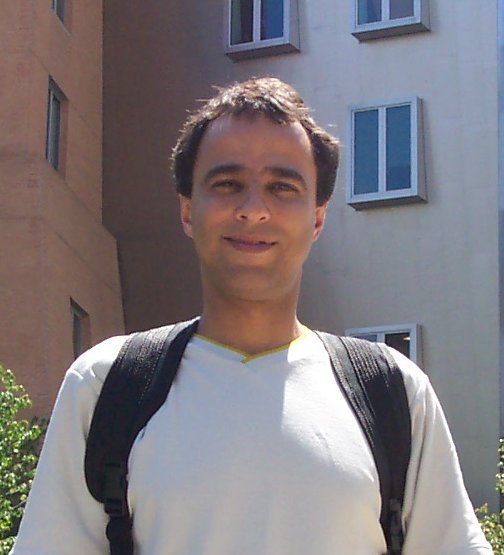
\includegraphics[width=.4\textwidth]{alfredo}
%
%            Alfredo Goldman \\
%            \emph{\alert{gold}@ime.usp.br} \\[.3cm]
%            \url{www.ime.usp.br/~gold} \\
%        \end{center}
%    \end{columns}
%\end{frame}

\subsection*{Index}

\begin{frame}
    \frametitle{Index}
    \setbeamertemplate{section in toc}[sections numbered]
    \tableofcontents[hideallsubsections]
\end{frame}

\begin{frame}
    \frametitle{Slides}
    \begin{center}
        
\includegraphics[width=.14\textwidth]{github}
    \end{center}
    The slides and all source code are hosted at \alert{GitHub}:

    \begin{itemize}
        \item \alert{Code \& Data}: \url{github.com/phrb/legup-tuner}
        \item \alert{Slides}: \url{github.com/phrb/slides-reconfig-2017-autotuning}
    \end{itemize}
\end{frame}

\section{FPGAs, HLS \& Autotuning}

\begin{frame}
    \frametitle{FPGAs}
    \begin{columns}[c,onlytextwidth]
        \column{0.55\textwidth}
        \begin{block}{FPGAs:}
        \begin{itemize}
            \item \alert{Logic Blocks} and \alert{Interconnections}
            \item \alert{Reconfigurable}
        \end{itemize}
        \end{block}

        \begin{block}{Tradeoff:}
        \begin{itemize}
            \item \alert{Energy Efficiency} and \alert{Performance}
            \item \alert{Programmability}
        \end{itemize}
        \end{block}

        \column{0.45\textwidth}
        \begin{center}
            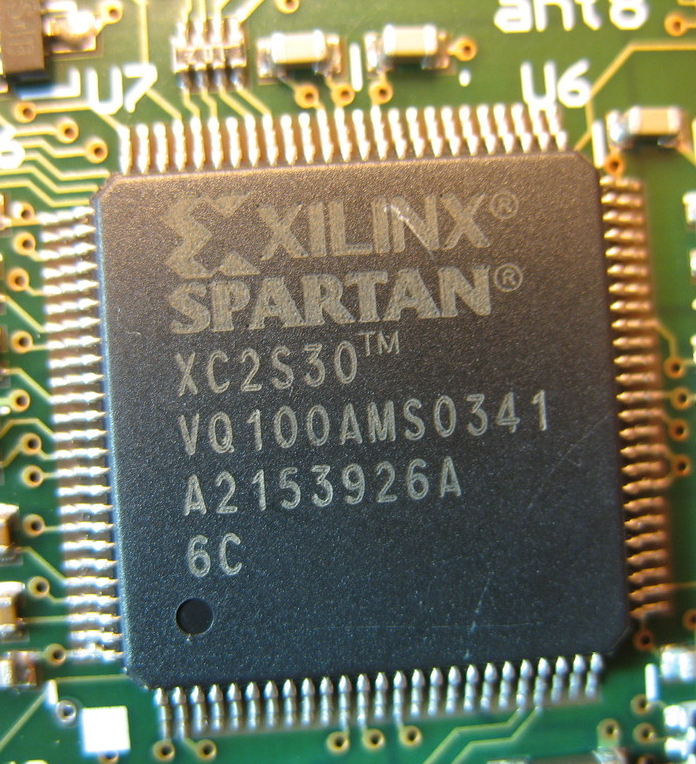
\includegraphics[width=.9\textwidth]{fpga}
        \end{center}
    \end{columns}
\end{frame}

\begin{frame}
    \frametitle{FPGAs}
    \begin{block}{Using FPGAs in \alert{Bing}:}
    \begin{center}
        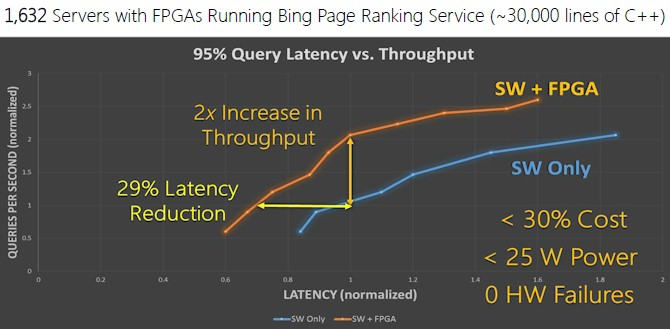
\includegraphics[width=.7\textwidth]{fpga_bing}

        \scriptsize{Image:
        \url{enterprisetech.com/2014/09/03/microsoft-using-fpgas-speed-bing-search/}
        [Accessed in 27/11/17]}
    \end{center}
    \end{block}
\end{frame}

\begin{frame}
    \frametitle{FPGAs: High-Level Synthesis}
    \begin{block}{\alert{LegUp} HLS flow:}
    \begin{center}
        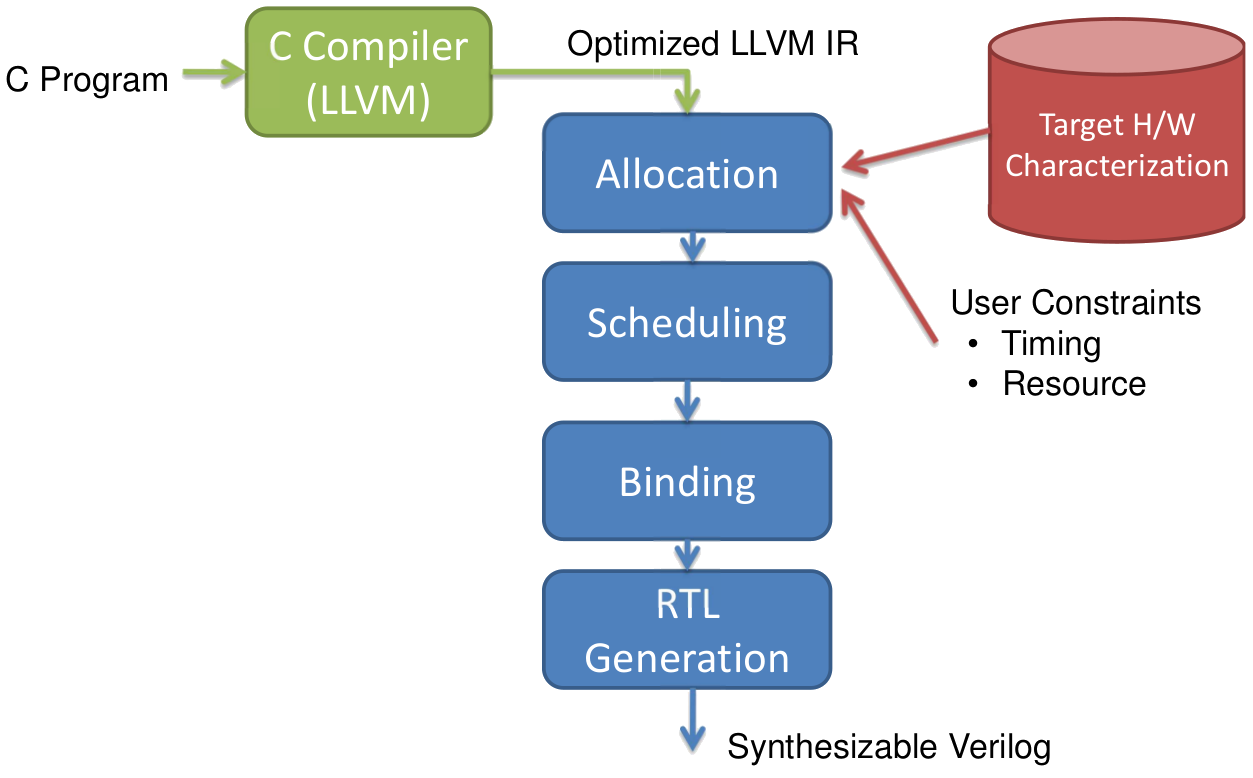
\includegraphics[width=.6\textwidth]{legup_flow}

        \scriptsize{Image: Canis, Andrew Christopher. LegUp: Open-Source
        High-Level Synthesis Research Framework. Diss. University of Toronto,
        2015.}
    \end{center}
    \end{block}
\end{frame}

\begin{frame}
    \frametitle{FPGAs: High-Level Synthesis}
    \begin{block}{HLS can generate \alert{lower-latency applications}:}
    \begin{center}
        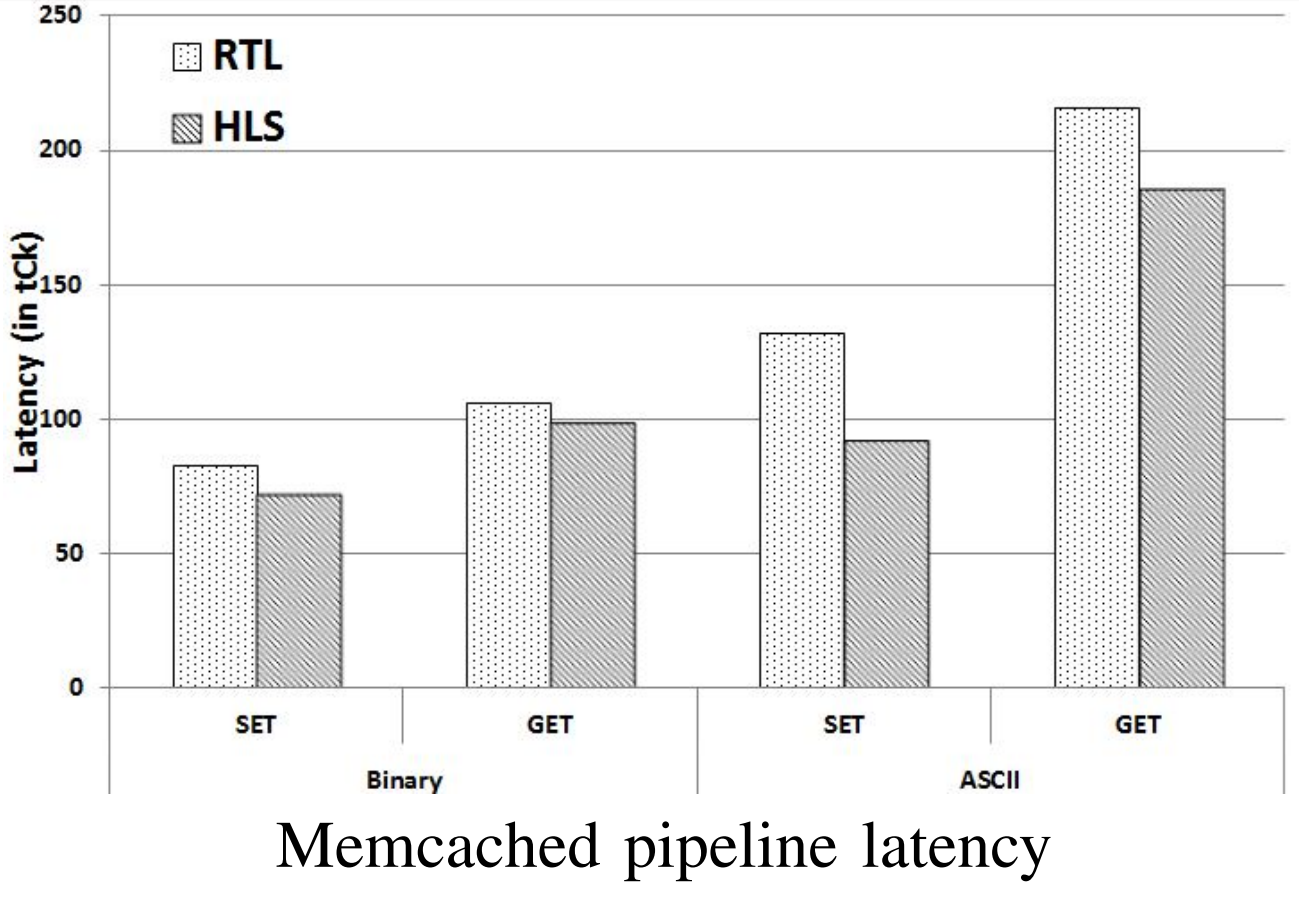
\includegraphics[width=.6\textwidth]{hls_latency}

        \scriptsize{Image: Karras, Kimon, Michaela Blott, and Kees Vissers.
        "High-Level Synthesis Case Study: Implementation of a Memcached
        Server." arXiv preprint arXiv:1408.5387 (2014).}
    \end{center}
    \end{block}
\end{frame}

\begin{frame}
    \frametitle{FPGAs: High-Level Synthesis}
    \begin{block}{\alert{Qualitatively}, with \alert{less effort}:}
    \begin{center}
        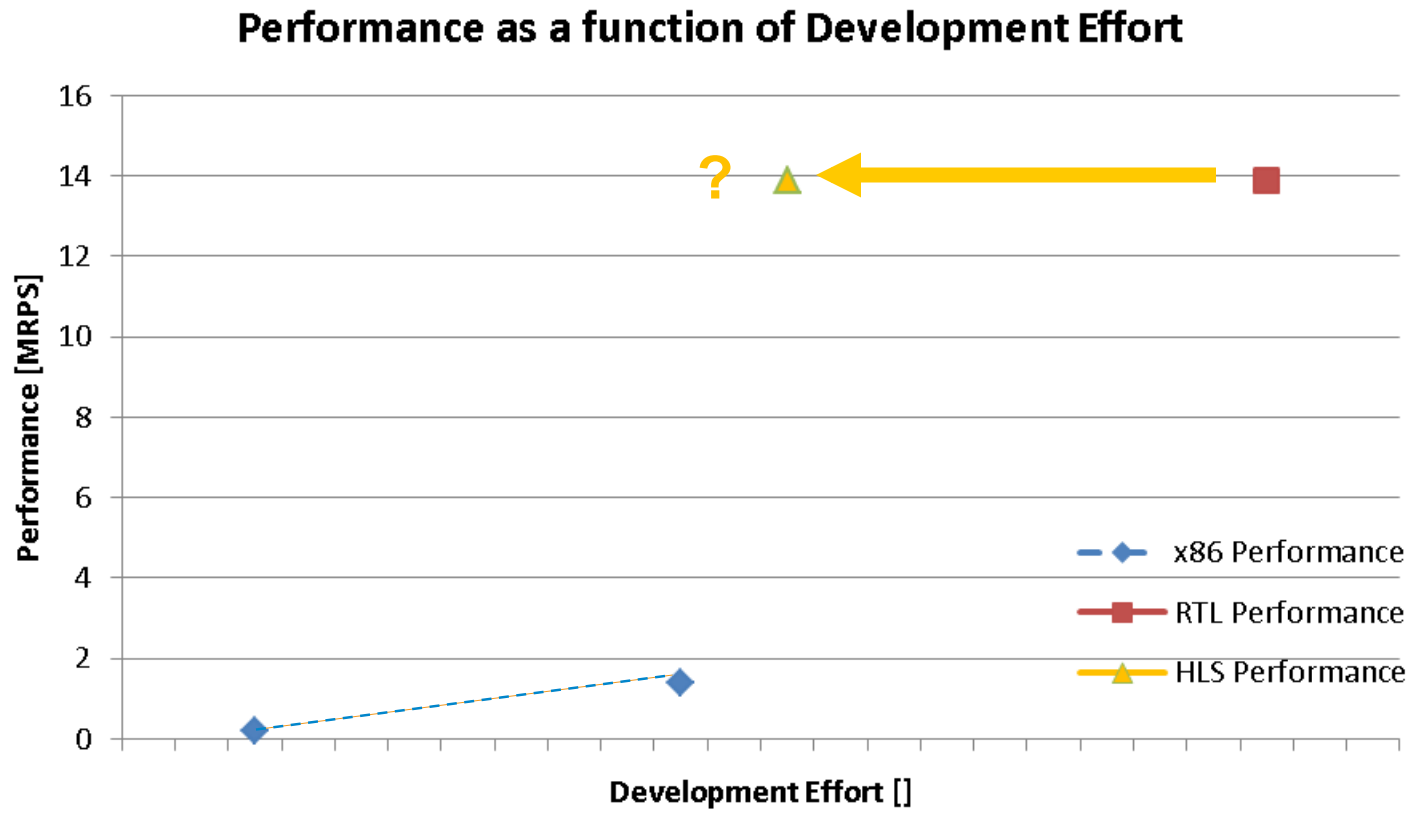
\includegraphics[width=.7\textwidth]{hls_loweffort}

        \scriptsize{Image: Blott, Michaela, et al. "Achieving 10Gbps line-rate
        key-value stores with FPGAs." Presented as part of the 5th USENIX
        Workshop on Hot Topics in Cloud Computing. 2013.}
    \end{center}
    \end{block}
\end{frame}

\begin{frame}
    \frametitle{FPGAs: High-Level Synthesis}
    \begin{block}{This is an \alert{old issue}:}
    \begin{center}
        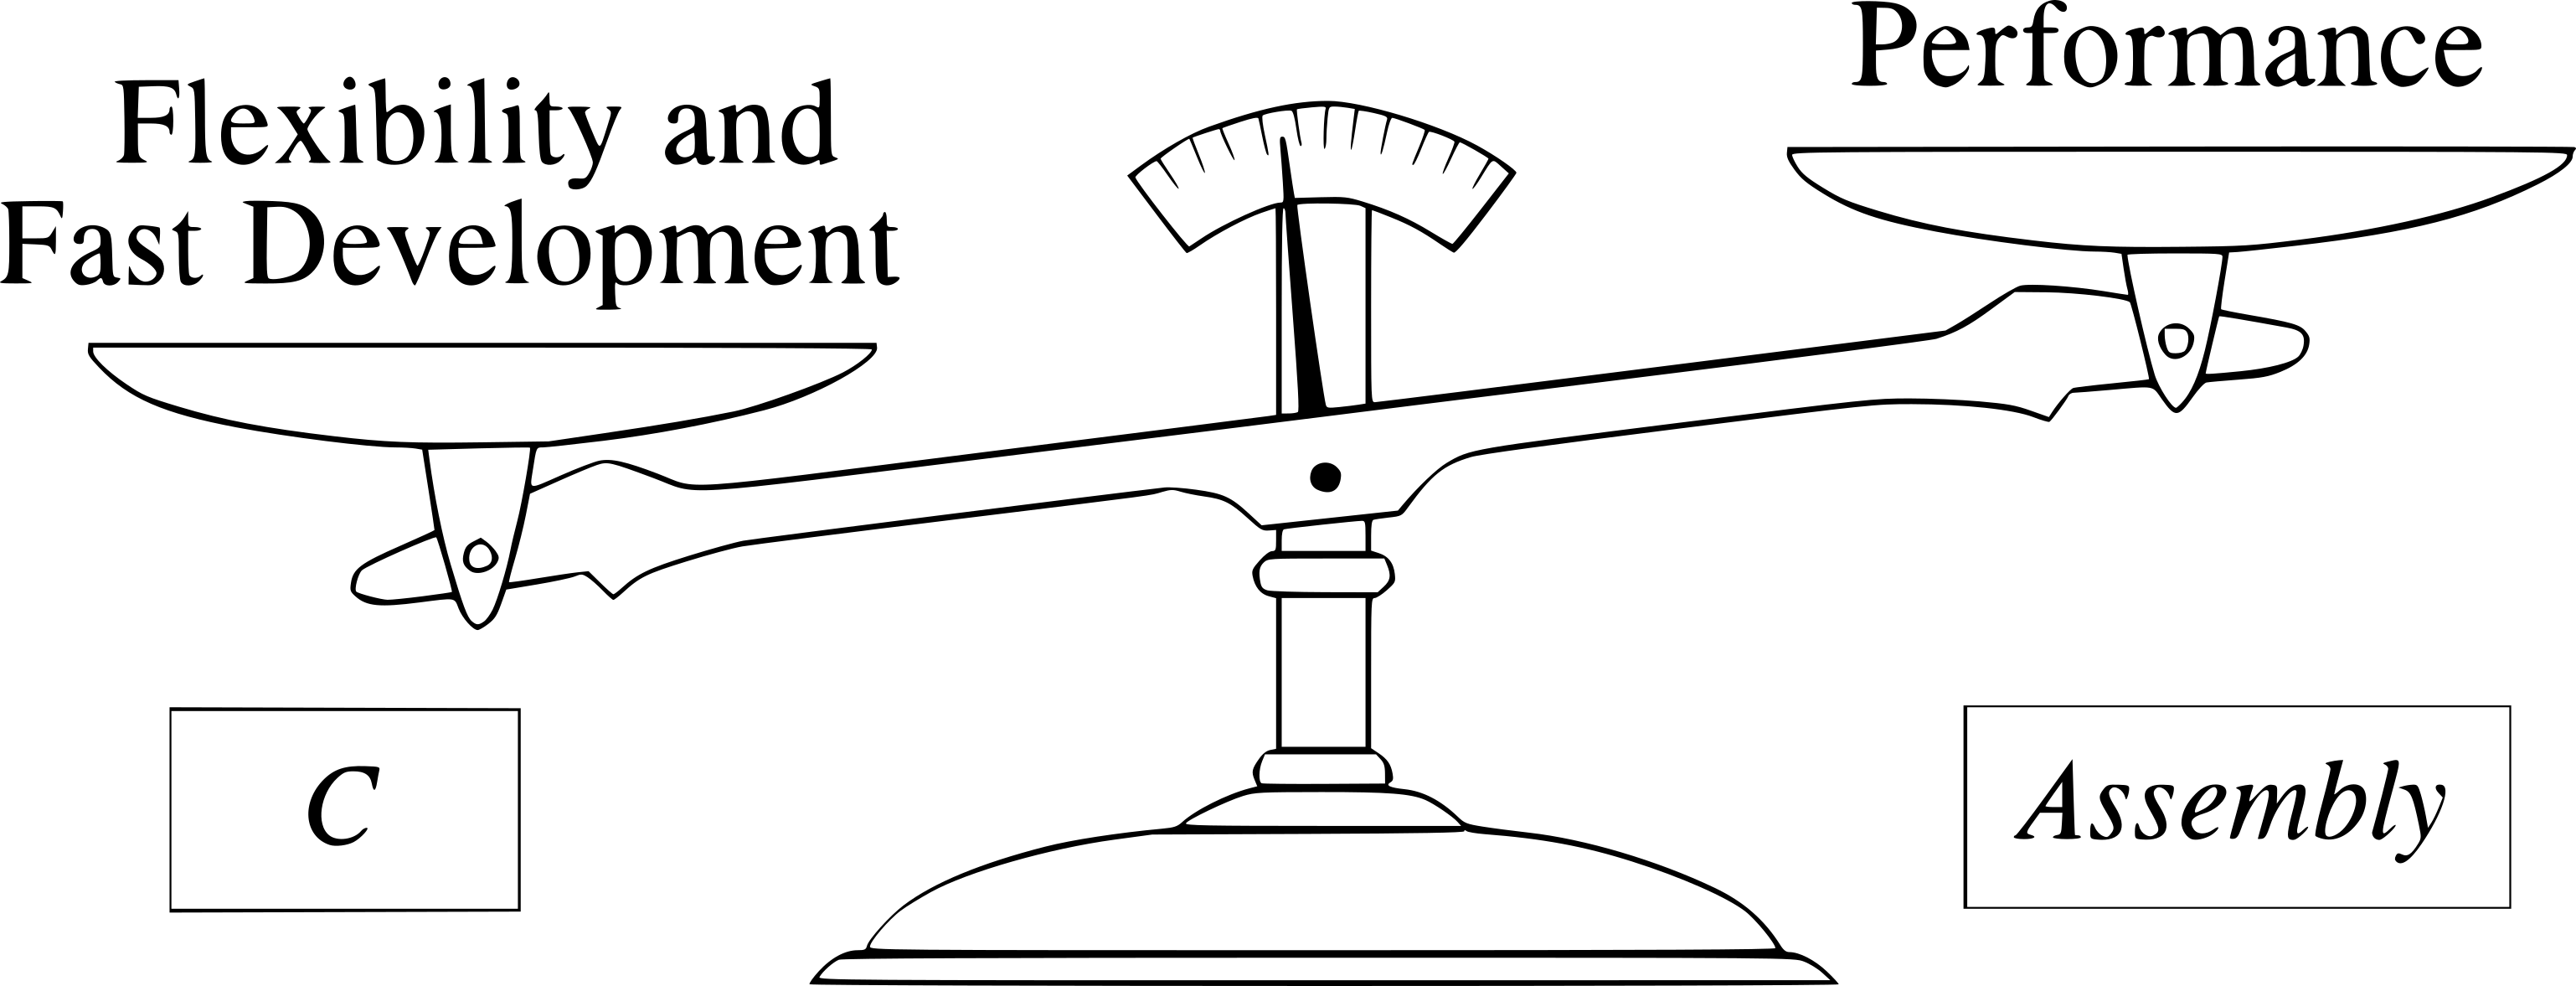
\includegraphics[width=.74\textwidth]{tradeoff_software}

        \scriptsize{Image: Smith, Steven W. "The scientist and engineer's guide
        to digital signal processing." 1997}
    \end{center}
    \end{block}
\end{frame}

\begin{frame}
    \frametitle{FPGAs: Autotuning}
    \begin{block}{Why use autotuning for HLS?}
    \end{block}
\end{frame}

\section{Background}

\begin{frame}
    \frametitle{Autotuning LLVM for HLS}
    \begin{block}{Compare with Huang's work}
    \end{block}
\end{frame}

\begin{frame}
    \frametitle{Autotuning Industry Designs for VTR}
    \begin{block}{Describe Xu's work with OpenTuner}
    \end{block}
\end{frame}

\section{Experiments \& Results}

\begin{frame}
    \frametitle{Benchmark and Hardware Metrics}
    \begin{block}{Describe CHStone and Metric Composition Strategy}
    \end{block}
\end{frame}

\begin{frame}
    \frametitle{Weighted Optimization Scenarios}
    \begin{block}{An \alert{Optimization Scenario} consists of:}
        \begin{itemize}
            \item An \alert{optimization objective}: \alert{performance}, \alert{area}, $\dots$
            \item \alert{Weights} for \alert{hardware metrics}
        \end{itemize}
    \end{block}

    \begin{block}{Our scenarios:}
        \begin{itemize}
            \item 3 \alert{specific} scenarios \& 1 \alert{balanced} scenario
            \item Weights: \alert{powers of two} from 1: \alert{irrelevant} to
                8: \alert{high}
        \end{itemize}
    \end{block}
\end{frame}

\begin{frame}
    \frametitle{Weighted Optimization Scenarios}
        \begin{table}[htpb]
            \caption{\alert{Weights} for \alert{Optimization Scenarios} (\alert{High} $= 8$, \alert{Medium} $= 4$, \alert{Low} $= 2$)}
            \centering
            \begin{tabular}{@{}lcccc@{}}
                \toprule
                Metric & \textit{Area} & \textit{Perf. \& Lat} & \textit{Performance} & \textit{Balanced} \\ \midrule
                \textit{LUT} & \cellcolor[HTML]{9B94B6} High & \cellcolor[HTML]{DD9583} Low & \cellcolor[HTML]{DD9583} Low & \cellcolor[HTML]{E3DBB3} Medium \\
                \textit{Registers} & \cellcolor[HTML]{9B94B6} High & \cellcolor[HTML]{9B94B6} High & \cellcolor[HTML]{E3DBB3} Medium & \cellcolor[HTML]{E3DBB3} Medium \\
                \textit{BRAMs} & \cellcolor[HTML]{9B94B6} High & \cellcolor[HTML]{DD9583} Low & \cellcolor[HTML]{DD9583} Low & \cellcolor[HTML]{E3DBB3} Medium \\
                \textit{DSPs} & \cellcolor[HTML]{9B94B6} High & \cellcolor[HTML]{DD9583} Low & \cellcolor[HTML]{DD9583} Low & \cellcolor[HTML]{E3DBB3} Medium \\
                \textit{FMax} & \cellcolor[HTML]{DD9583} Low & \cellcolor[HTML]{9B94B6} High & \cellcolor[HTML]{9B94B6} High & \cellcolor[HTML]{E3DBB3} Medium \\
                \textit{Cycles} & \cellcolor[HTML]{DD9583} Low & \cellcolor[HTML]{9B94B6} High & \cellcolor[HTML]{DD9583} Low & \cellcolor[HTML]{E3DBB3} Medium \\ \bottomrule
            \end{tabular}
        \end{table}
\end{frame}

\begin{frame}
    \frametitle{Results}
    \begin{block}{Present the heatmaps for each optimization scenario}
    \end{block}
\end{frame}

\section{Conclusion}

\begin{frame}
    \frametitle{Limitations of this Work}
    \begin{block}{Discuss the issues with the weighted cost function}
    \end{block}
\end{frame}

\begin{frame}
    \frametitle{Future Work}
    \begin{block}{Discuss all future work topics}
    \end{block}
\end{frame}

\maketitle

\end{document}
